
Having examined which feedback variables to retain under single-node actuation, we next assess the complementary resource choice: the number of actuators. To quantify the performance cost of restricting actuation to one node, nominal PPO synchronization is evaluated for every nonempty subset of the three nodes: $\{1\}$, $\{2\}$, $\{3\}$, $\{1,2\}$, $\{1,3\}$, $\{2,3\}$, and $\{1,2,3\}$. For a subset $\mathcal S$, the input matrix contains the corresponding columns of $I_3$, and the policy produces $|\mathcal S|$ actions. The six-dimensional observation, error-only reward, initial-state distribution, RK4 integration, policy hidden layers, PPO hyperparameters, and nominal training budget of $4\times10^5$ transitions are unchanged. Each configuration includes three independent training runs and is evaluated on 20 common test initial conditions. All seven configurations and all three final checkpoints per configuration are reported, including configurations with poor synchronization.

The same per-actuator bound $|u_j|\leq4$ is imposed in every configuration, while $E_u$ sums energy across all active channels. Thus, additional actuators provide both additional control directions and a larger admissible total input magnitude ($\|\mathbf u\|_2\leq4\sqrt{|\mathcal S|}$). The comparison therefore measures the joint effect of additional control directions and increased aggregate control authority. Only nominal synchronization is tested in this ablation. Actuator count quantifies the structural actuation requirement.

\input{generated/multi_input_table_ASC.tex}

\begin{figure*}[pos=!t,width=\textwidth]
  \centering
  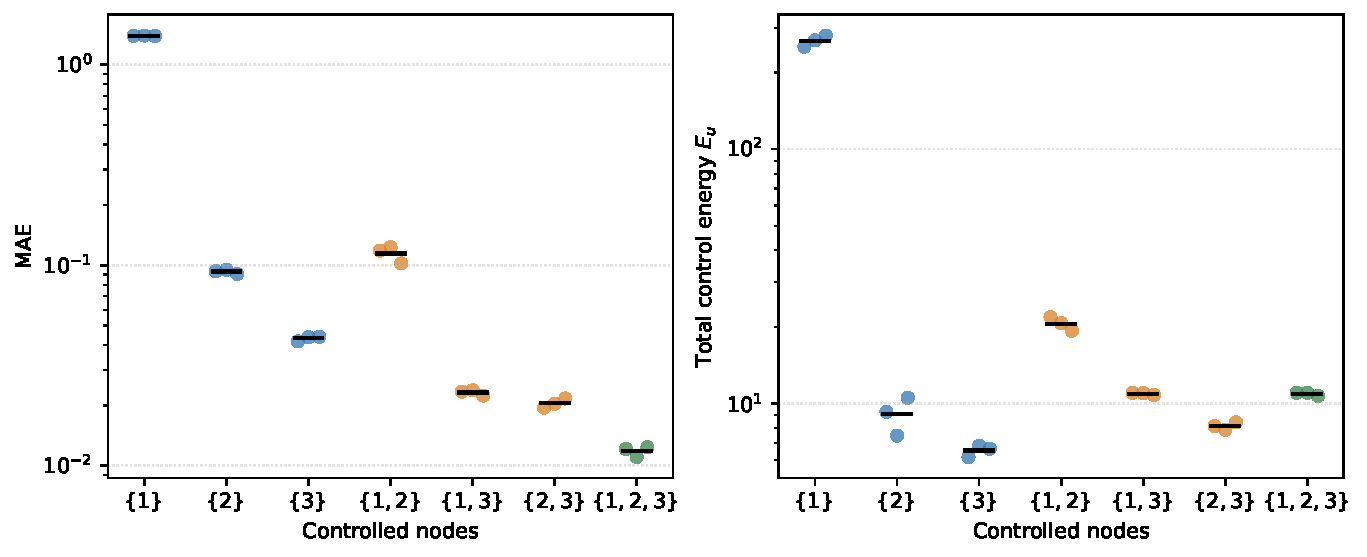
\includegraphics[width=\textwidth]{figures/multi_input_matched_budget.pdf}
  \caption{Nominal synchronization error and total control energy for all actuator subsets. Each colored point is a training-seed mean over 20 common test initial conditions; black horizontal marks denote the mean across three seeds. Blue, orange, and green indicate one, two, and three actuators, respectively.}
  \label{fig:multi_input_comparison}
\end{figure*}

Table~\ref{tab:multi_input_comparison} and Fig.~\ref{fig:multi_input_comparison} quantify the tradeoff. Single-node control at Node 3 gives MAE 0.0431 and energy 6.54, whereas $\{2,3\}$ gives 0.0205 and 8.15 and $\{1,2,3\}$ gives 0.0118 and 10.91. Thus, one actuator retains low-residual synchronization with lower measured energy, but incurs a higher full-horizon error than these multi-input configurations. The steady L1 error does not decrease monotonically with actuator count: it is 0.0091 for $\{3\}$, compared with 0.0141 for $\{2,3\}$ and 0.0105 for $\{1,2,3\}$. Full-horizon accuracy and steady-state precision thus capture different consequences of increasing actuator availability.

The $\{1,2\}$ configuration has higher MAE and energy than $\{2\}$ under the fixed training budget, while configurations containing Node 3 perform better in full-horizon MAE. This emphasizes the effect of actuator placement and finite-budget policy optimization. Although adding an actuator enlarges the admissible control set, exploiting that flexibility also depends on policy optimization within the available training budget. These results quantify the accuracy--effort tradeoff of single-input control as a resource-constrained design choice.
